
\documentclass[12pt]{article}
\usepackage{geometry}
\usepackage{pgfplots}
\usepackage{tabularx}
\usepackage{array}
\usepackage{multirow}
\usetikzlibrary{arrows,positioning,automata,arrows.meta, shapes.geometric,decorations.pathreplacing, calc}
\usepackage{tikz}
\geometry{top=1in, bottom=1in, left=1in, right=1in}
\setlength{\parindent}{0pt}

\definecolor{headercolor}{RGB}{142, 180, 227} 
\definecolor{rowcolor}{RGB}{230, 240, 255}  

\newcolumntype{L}{>{\raggedright\arraybackslash}p{0.5\textwidth}}
\newcolumntype{R}{>{\raggedleft\arraybackslash}p{0.5\textwidth}}


\begin{document}

\begin{figure}[ht]
\caption{Fitted SEM for two people deciding whether or not to watch a movie.}
\centering
\textbf{Simulations Run}: 5\\
\textbf{Agents}: [`person 1', `person 2']\\

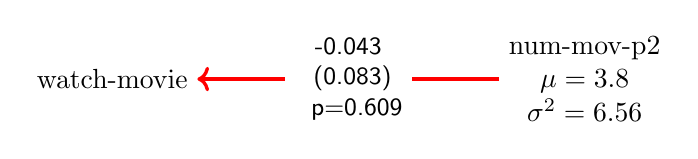
\begin{tikzpicture}
    \pgfdeclarelayer{background}
    \pgfdeclarelayer{foreground}
    \pgfsetlayers{background,main,foreground}
    \node[align=center] (watch-movie) at (0,0) {watch-movie};
\node[align=center] (num-mov-p2) at (0:6cm) {num-mov-p2\\ $\mu = 3.8$ \\ $\sigma^2 = 6.56$};
\begin{pgfonlayer}{background}
\draw[->,red,very thick] (num-mov-p2) -- (watch-movie);
\end{pgfonlayer}
\begin{pgfonlayer}{foreground}
\path (num-mov-p2) -- (watch-movie) node[midway, fill=white, font=\sffamily\small, align=center] {-0.043\\\phantom{-}(0.083)\\\phantom{-} p=0.609 };
\end{pgfonlayer}
\end{tikzpicture}\
  \begin{minipage}{\textwidth}
    \begin{footnotesize}
      \emph{Notes:} Each exogenous cause is given with its mean and variance. 
       The edges are labeled with their unstandardized path estimate, standard error, and p-value. 
    \end{footnotesize}
    \end{minipage}
\end{figure}
\end{document}
